\documentclass{beamer}

\usetheme{CambridgeUS}
\usecolortheme{beaver}

\usepackage[utf8]{inputenc}
\usepackage[brazil]{babel}
\usepackage{caption}
\usepackage{hyperref}
\hypersetup{
    bookmarks=true,         % show bookmarks bar?
    unicode=false,          % non-Latin characters in Acrobat’s bookmarks
    pdftoolbar=true,        % show Acrobat’s toolbar?
    pdfmenubar=true,        % show Acrobat’s menu?
    pdffitwindow=false,     % window fit to page when opened
    pdfstartview={FitW},    % fits the width of the page to the window
    pdftitle={Introdução ao \LaTeX com o Overleaf},    % title
    pdfauthor={Nightwind},     % author
    pdfsubject={Introdução ao Overleaf},   % subject of the document
    % pdfcreator={Creator},   % creator of the document
    % pdfproducer={Producer}, % producer of the document
    pdfkeywords={latex, dicas}, % list of keywords
    pdfnewwindow=true,      % links in new PDF window
    colorlinks=false,       % false: boxed links; true: colored links
    linkcolor=red,          % color of internal links (change box color with linkbordercolor)
    citecolor=green,        % color of links to bibliography
    filecolor=cyan,         % color of file links
    urlcolor=magenta        % color of external links
}
\usepackage[style=abnt]{biblatex}
\addbibresource{references.bib}
\usepackage{csquotes}

\title{Utilizando o Overleaf}
\author{Nightwind}
\institute[CTISM]{Colégio Técnico Industrial de Santa Maria}
\logo{
\includegraphics[width=1cm]{../images/photo1.jpg}}
\date{\today}

\begin{document}

    \frame{\titlepage}

    \begin{frame}
        \frametitle{Sumário}
        \tableofcontents
    \end{frame}

    \section[Página Inicial]{Página Inicial do Overleaf}
    \begin{frame}
        \frametitle{Homepage}
    \begin{figure}
        \centering
        \caption[HomePage]{Página Inicial do Overleaf.}
        \label{fig:homepageOverleaf}
        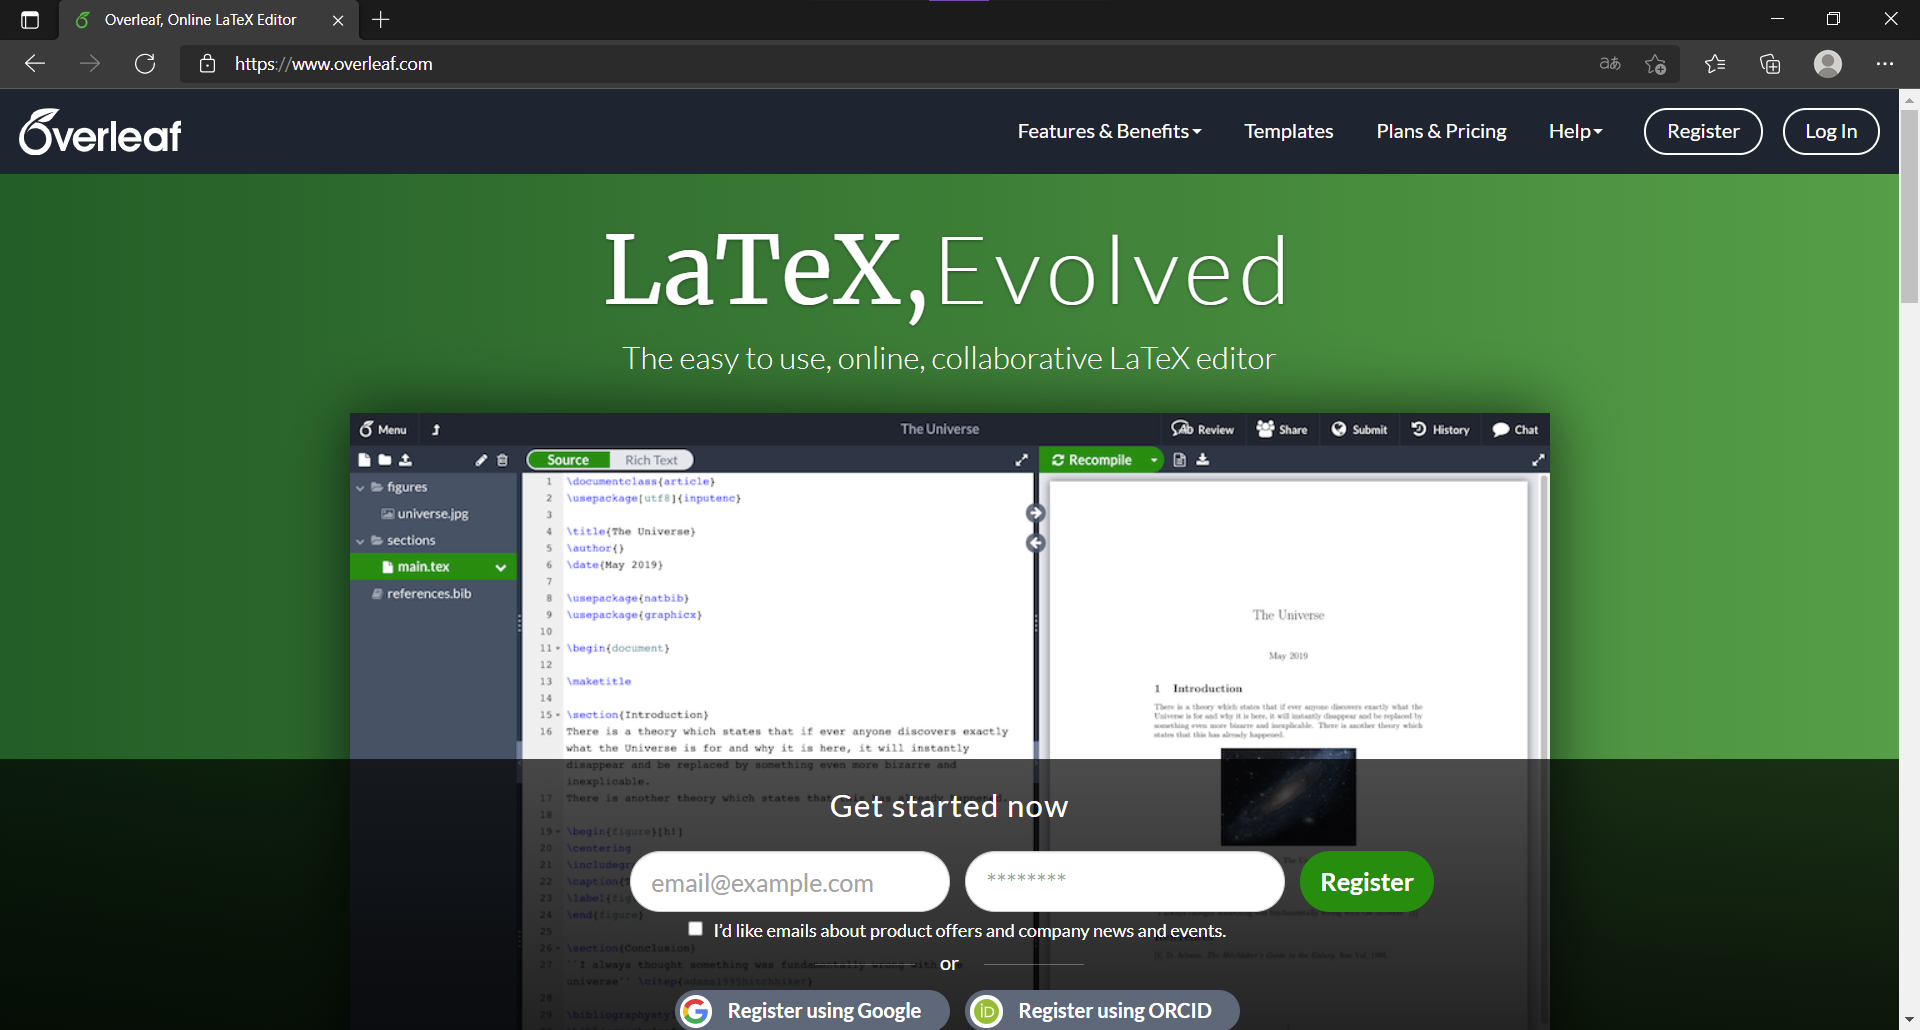
\includegraphics[width=0.8\textwidth]{../images/homepageOverleaf.png}
        \caption*{\footnotesize \url{https://www.overleaf.com/}}
    \end{figure}    
    \end{frame}

    \begin{frame}
        \frametitle{Homepage}
    \begin{itemize}
        \item Vá em ``\textit{Register}'' caso ainda não tenha uma conta.
        \item Vá em ``\textit{Log In}'' caso já tenha uma conta. 
        \item Coloque \textit{e-mail} e senha.
    \end{itemize}
    \end{frame}
        
    \section{Área do Usuário}
    \begin{frame}
        \frametitle{Novo usuário}
    \begin{figure}
        \centering
        \caption{Área do novo usuário.}
        \label{fig:newUserOverleaf}
        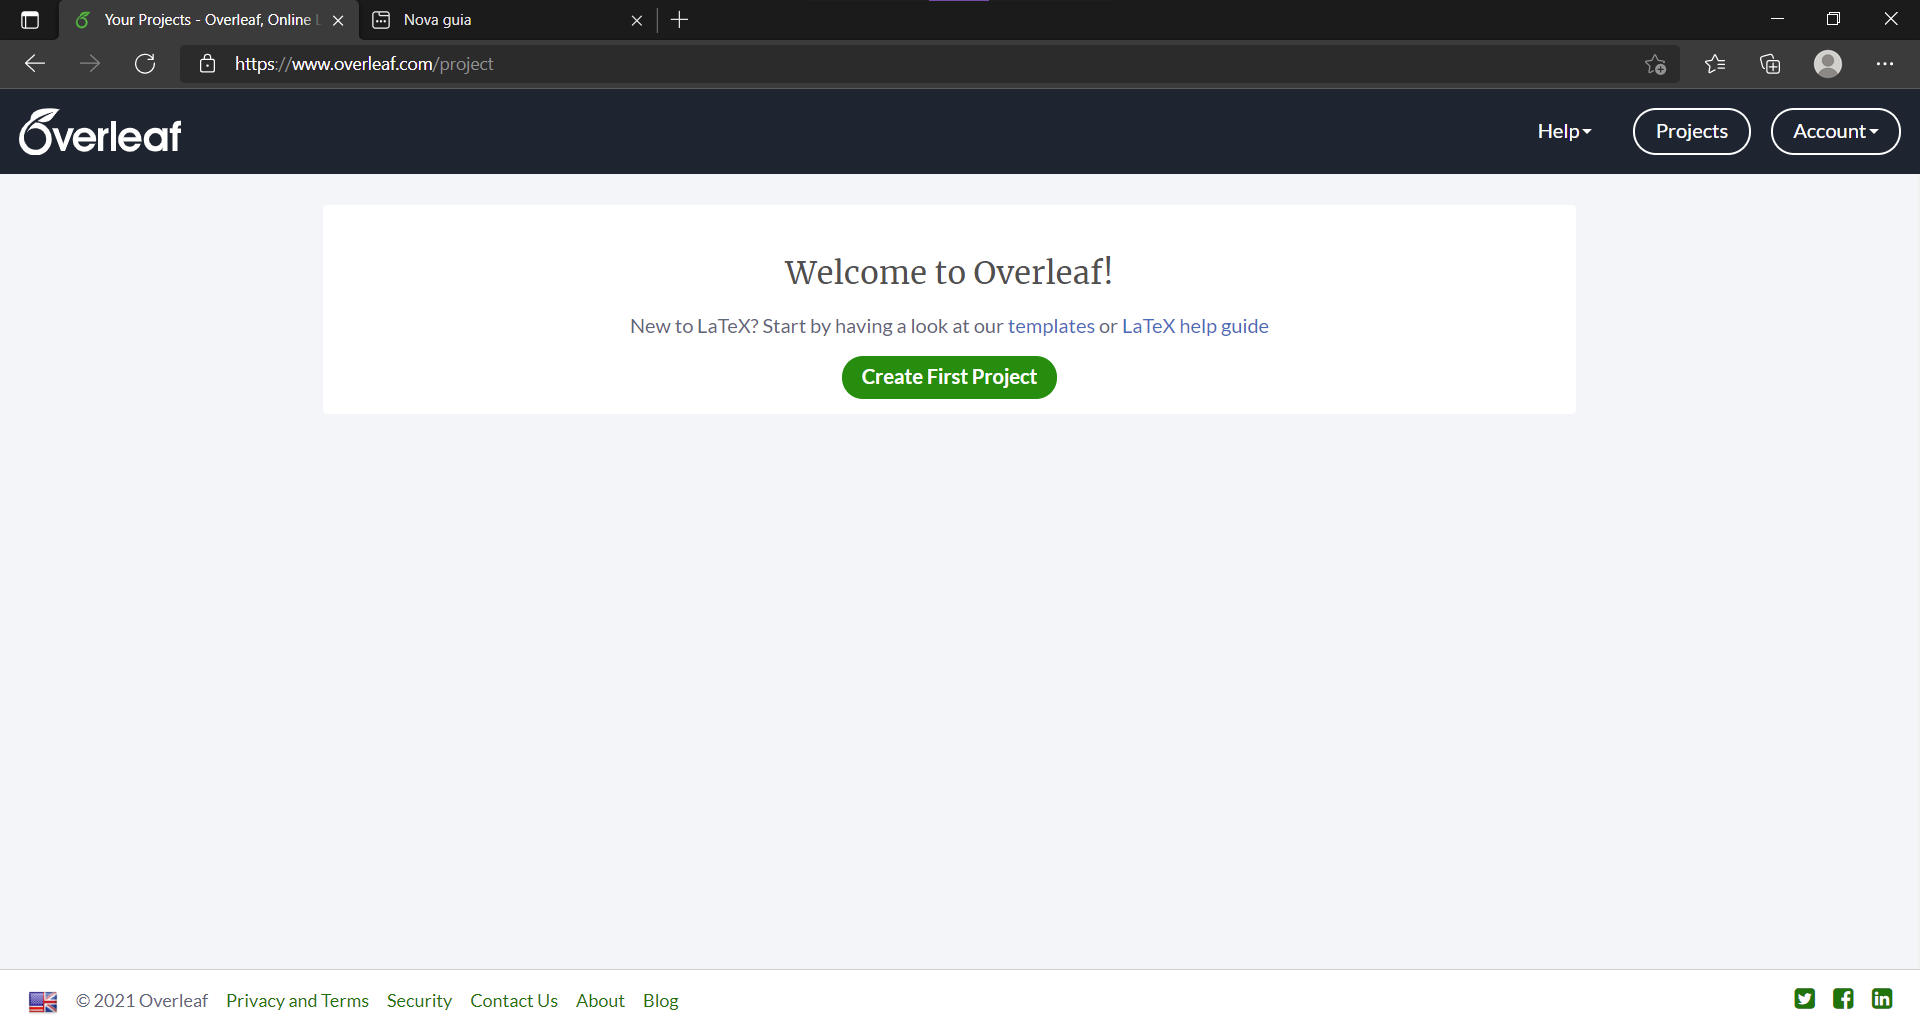
\includegraphics[width=0.8\textwidth]{../images/newUserOverleaf.png}
    \end{figure}
    \end{frame}

    \begin{frame}
        \frametitle{Primeiro Documento}
    \begin{columns}
        \begin{column}{0.5\textwidth}
            \begin{itemize}
                \item Para novos usuários, o \href{https://www.overleaf.com/}{Overleaf} recomenda visualizar os \href{https://www.overleaf.com/latex/templates}{Templates} e o \href{https://www.overleaf.com/learn}{Guia de \LaTeX}. Ambos são altamente recomendáveis. 
                \item Para criar o primeiro projeto, clicar em ``\textit{Create First Project}''.
                \item Uma lista de opções aparecerá, como mostra a \autoref{fig:createANewProject}.
            \end{itemize} 
        \end{column}
        \begin{column}{0.5\textwidth}
            \begin{figure}
                \centering
                \caption{Opções de Projeto.}
                \label{fig:createANewProject}
                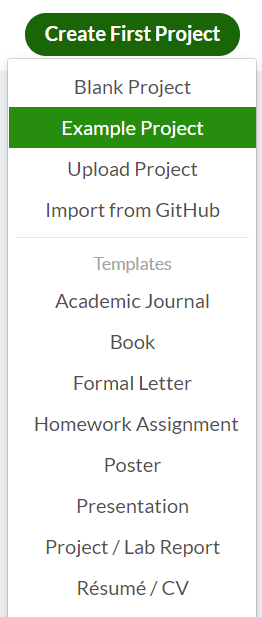
\includegraphics[width=0.3\textwidth]{../images/createANewProject.png}
            \end{figure}
        \end{column}
    \end{columns}  
    \end{frame}

    \section{Novo documento}

    \begin{frame}
        \frametitle{Novo documento}
    \begin{itemize}
        \item Para fins de ilustração, a opção escolhida foi ``\textit{Blank Project}''.
    \end{itemize}
        
    
    \end{frame}

    \begin{frame}
        \frametitle{Novo documento}
        \begin{figure}
            \centering
            \caption{Nomeando um novo documento.}
            \label{fig:nameOfProject}
            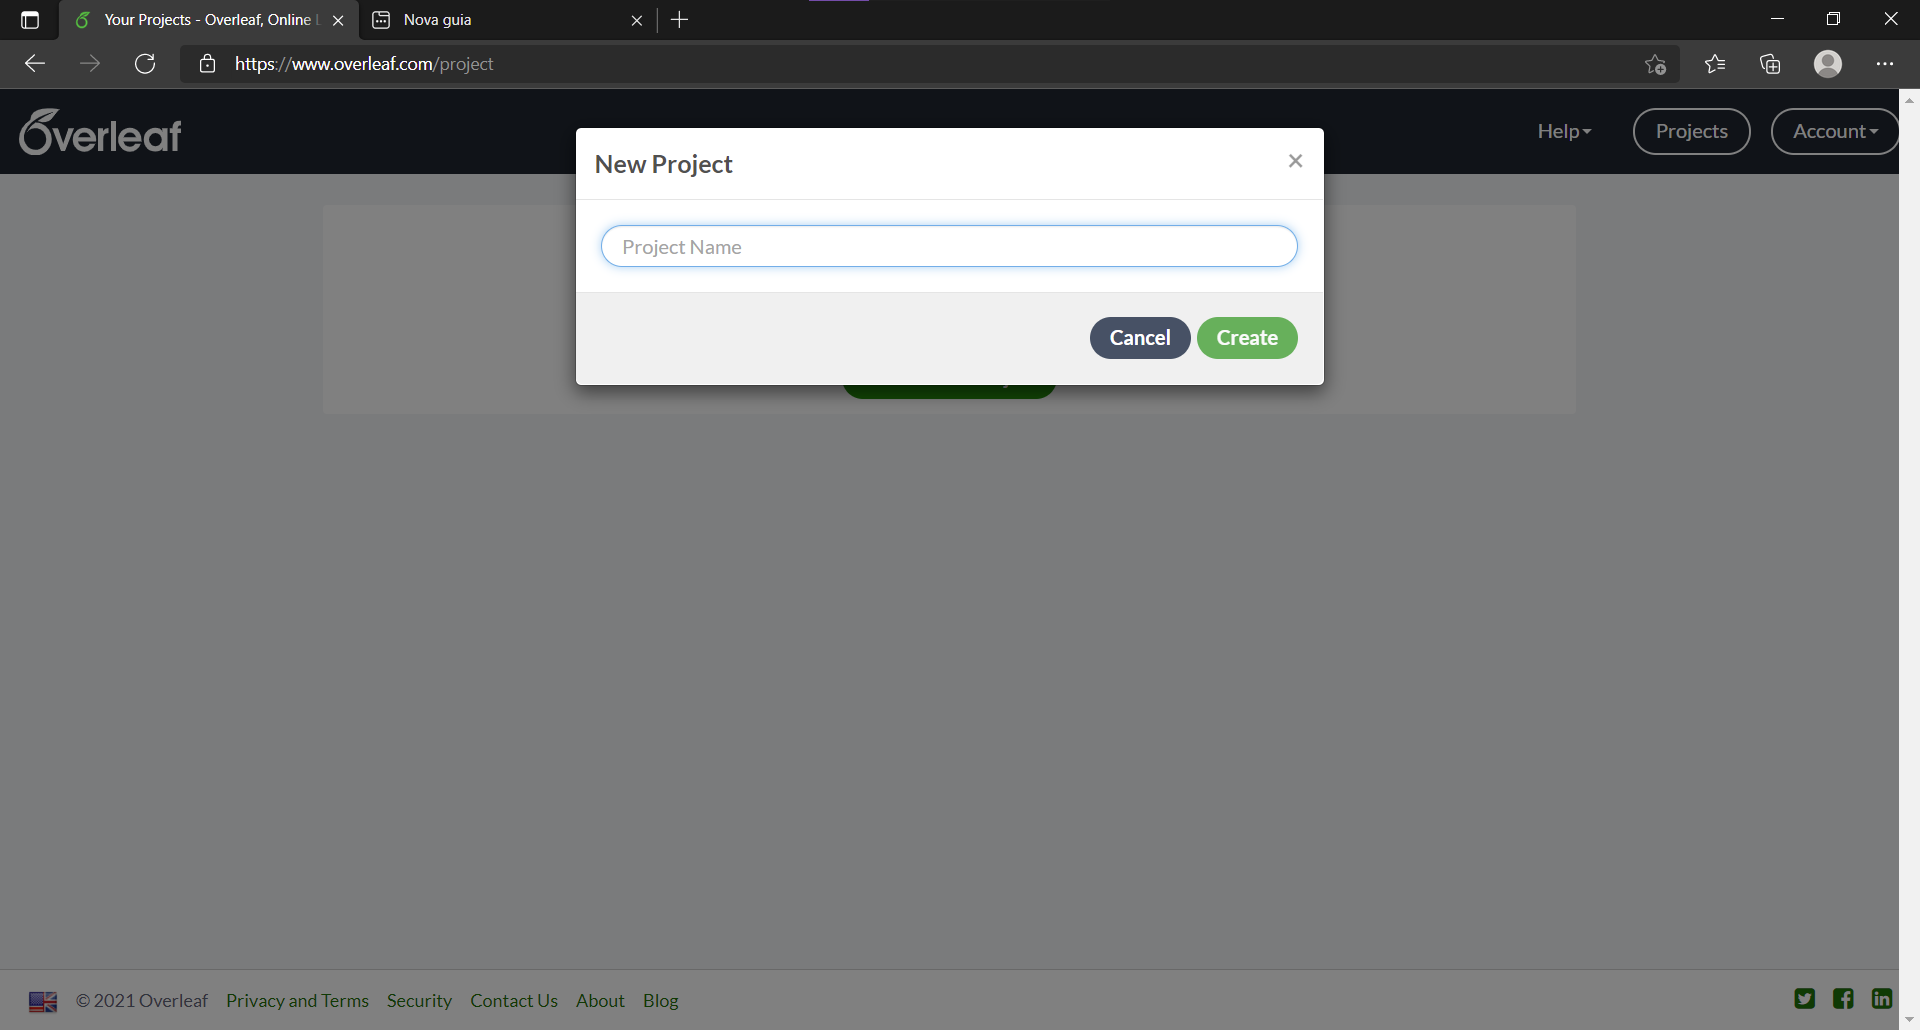
\includegraphics[width=0.8\textwidth]{../images/nameOfProject.png}
        \end{figure}
    \end{frame}

    \begin{frame}
        \frametitle{Novo documento}
    \begin{itemize}
        \item Depois de dar o nome da sua preferência, clique em ``\textit{Create}''.
    \end{itemize}    
    \end{frame}

    \begin{frame}
        \frametitle{Novo documento}
        \begin{figure}
            \centering
            \caption{Documento em branco.}
            \label{fig:blankProject}
            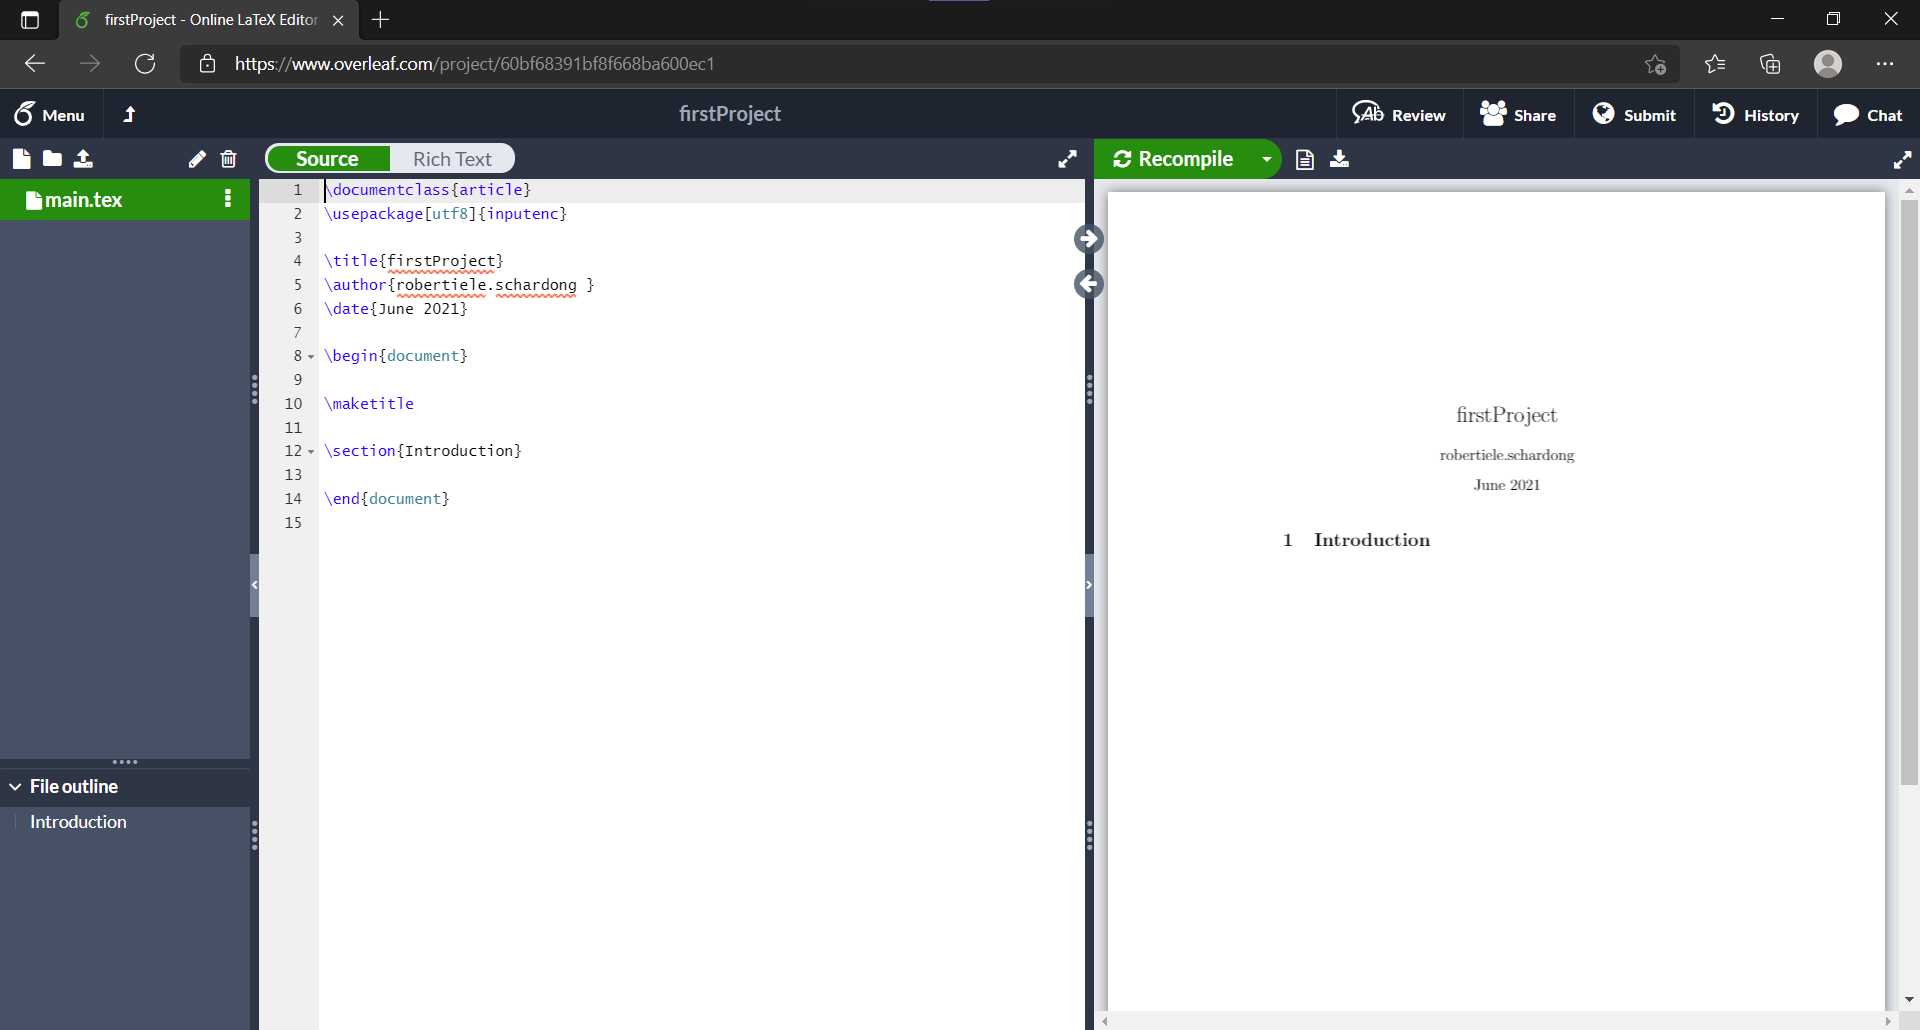
\includegraphics[width=0.8\textwidth]{../images/blankProject.png}
        \end{figure}    
    \end{frame}

    \begin{frame}
        \frametitle{Referências}
        \nocite{overleafBeamer,overleafDocumentation,overleafTemplates}
        \printbibliography[]{}
    \end{frame}
\end{document}
